\documentclass[8pt]{beamer}

\usetheme{Madrid}
\usepackage{amsmath, amssymb, amsthm}
\usepackage{xcolor}
\usepackage{syntax}
\usepackage{stmaryrd}
\usepackage{multicol}
\usepackage{biblatex}
\usepackage{ulem}
\usepackage{tikz}
\addbibresource{ref.bib}

\usepackage{tikz}
\usepackage{graphicx}
\graphicspath{{figures/}, {impl/simulation-results/}}
\DeclareGraphicsExtensions{.png,PNG,.jpg,.JPG,.jpeg,.JPEG,.pdf,.PDF}
\usepackage{subcaption}
\usepackage{amsmath, amsthm, amssymb}

\DeclareMathOperator*{\argmax}{arg\,max}
\DeclareMathOperator*{\argmin}{arg\,min}

\DeclareMathOperator*{\PGF}{PGF}
\DeclareMathOperator*{\SOP}{SOP}
\DeclareMathOperator*{\VARS}{Var}
\DeclareMathOperator*{\PARMS}{Param}
\DeclareMathOperator*{\iid}{iid}
\DeclareMathOperator*{\lfp}{fix}
\renewcommand{\S}[1]{ \llbracket #1 \rrbracket }
\newcommand{\E}{ \mathbb{E} }

\title{PGF transformer semantics}
\author{Cheng Peng \and Dantong Liu\thanks{External collaborator, BME undergrad at ShanghaiTech}}
\date{\today}

\AtBeginSection[] % Do nothing for \section*
{
	\begin{frame}<beamer>
		\frametitle{Contents in this section}
		\begin{multicols}{2}
		\tableofcontents[currentsection]
		\end{multicols}
	\end{frame}
}

\newcommand{\verbatimfont}[1]{\renewcommand{\verbatim@font}{\ttfamily\tiny}}

% 10 minutes presenting
% 5 minutes Q&A
\begin{document}

\maketitle

\begin{frame}[fragile, allowframebreaks]{Motivating Example: Knuth-Yao Dice}
	\begin{verbatim}
nat s; nat die;

while (s < 7) {
         if(s = 0) { { s:=1 }[1/2]{ s:=2 } }
  else { if(s = 1) { { s:=3 }[1/2]{ s:=4 } }
  else { if(s = 2) { { s:=5 }[1/2]{ s:=6 } }
  else { if(s = 3) { { s:=1 }[1/2]{ s:=7; die:=1 } }
  else { if(s = 4) { { s:=7; die:=2 }[1/2]{ s:=7; die:=3 } }
  else { if(s = 5) { { s:=7; die:=4 }[1/2]{ s:=7; die:=5 } }
  else { if(s = 6) { { s:=2 }[1/2]{ s:=7; die:=6 } }
  else { skip } } } } } } } }
		\end{verbatim}

	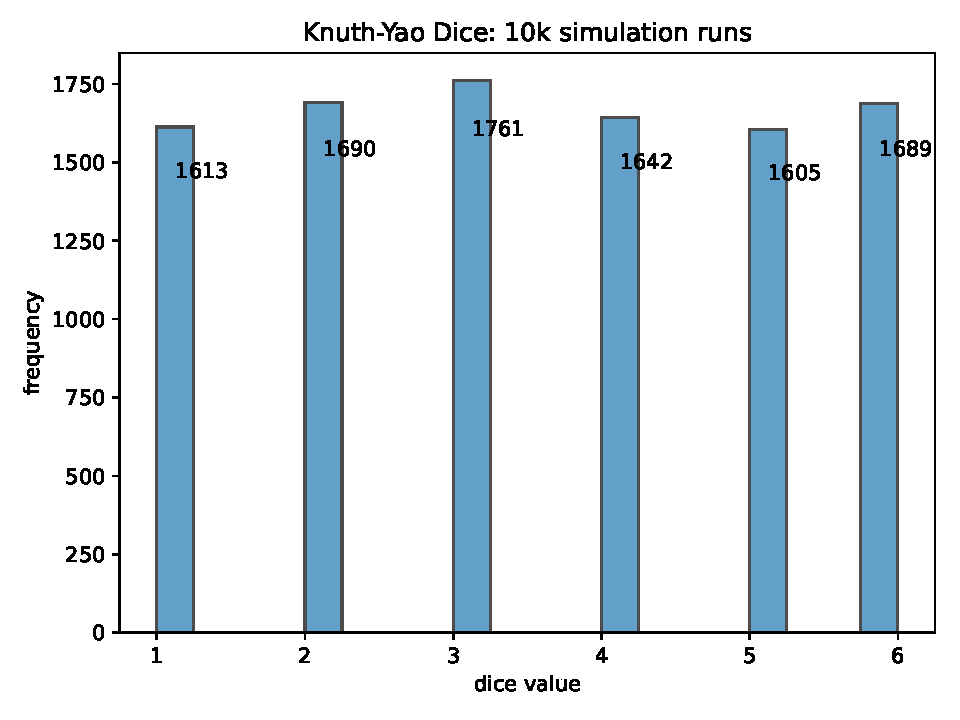
\includegraphics[width=0.5\textwidth]{ky-die-bars}\\
	\verb|die := unif(1,6);|
\end{frame}

\begin{frame}{The main theme}
	PGF transform semantics based equivalence checking of pGCL programs.
	\begin{enumerate}
		\item A denotational semantics capturing the dynamics of all possible executions.
		\item The specification will be given as a pGCL program.
		\item Focus on a linear fragment of pGCL, called ReDiP.
	\end{enumerate}
	\hfill
	\begin{block}{Remarks}
		\begin{itemize}
			\item Equivalence checking of pGCL is undecidable
			\item Linearity. No normalization is involved.
		\end{itemize}
	\end{block}
\end{frame}

\section{Introduction}
\subsection{Backgrounds}
\begin{frame}{Backgrounds}
	\begin{block}{The rise of probabilistic programming}
		Randomness is ineluctable.
		\begin{itemize}
			\item Simulating the physics world.
			\item Building statistical models.
			\item Deriving efficient approximate algorithms.
		\end{itemize}
	\end{block}
	\begin{block}{The need to verify stochastic programs}
		Your property and life are at stake.
		\begin{itemize}
			\item Security-critical applications: cryptography systems
			\item Safety-critical applications: cyber-physics systems
		\end{itemize}
		A trust problem: simulation can demonstrate unreliability but not prove reliability.
	\end{block}
\end{frame}
\subsection{Limitations of previous works}
\begin{frame}{Insufficiency of previous works}
	\begin{exampleblock}{matured approaches}
		\begin{itemize}
			\item Evaluating moments of variables\cite{wang2021central}
			\item Deriving assertion violation probability\cite{assert}
			\item Establishing lower/upper bounds\cite{probana}
		\end{itemize}
	\end{exampleblock}
	\begin{block}{insufficiency}
		\begin{itemize}
			\item Sensitivity to slight perturbation.
			\item Expressiveness: marginal/conditional. tail/concentration. parameter synthesis.
		\end{itemize}
	\end{block}

	Our goal: to enable precise and versatile verification
\end{frame}

\section{Overview}
\begin{frame}{Overview of the solution}
	\begin{description}
		\item[Input program] A program in ReDiP, a fragment of pGCL
		\item[Specification program] A \emph{loop-free} ReDiP program: distribution of the \emph{final} program state
		\item[Loop invariants] Fixed point of loops, encoded as ReDiP programs.
		\item[Verifier] check semantic equivalence, where the semantics of a program is
		      \begin{itemize}
			      \item A computational tree of configurations and transitions.
			      \item A mhapping from initial configuration to a distribution of output states.
			      \item A (linear) transformer maps a PGF to another PGF.
		      \end{itemize}
		\item[Output] True/False.
	\end{description}
\end{frame}

\section{pGCL and ReDiP}
\subsection{Syntax and Semantics of pGCL}
\begin{frame}[allowframebreaks]{Syntax and Semantics of pGCL\cite{pgcl}}
	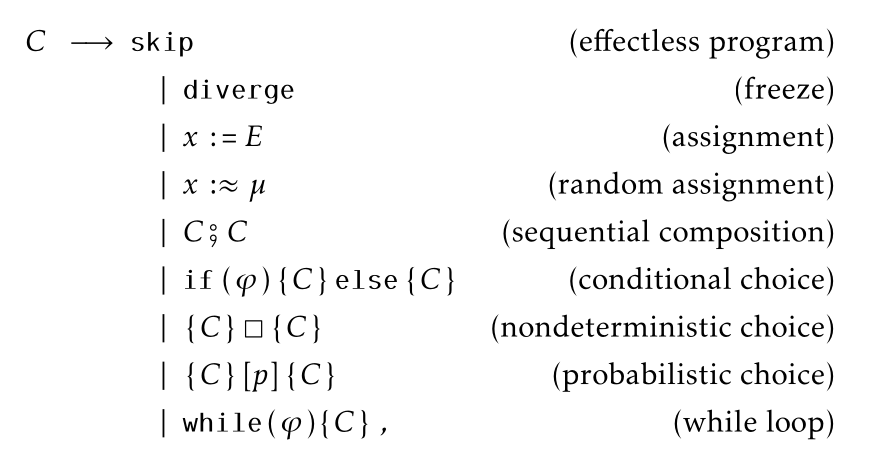
\includegraphics[width=0.8\textwidth]{pgcl}
	\begin{description}
		\item[configuration] \(\mathcal{K} = \langle C,\sigma,n,\theta,\eta,q\rangle\).
		\item[transition relation] \(\vdash \subseteq \mathbb{K}\times\mathbb{K}\).
		\item[computational tree] (initial configurations, reachable configuration, transitions).
	\end{description}
	\framebreak
	\begin{columns}
		\begin{column}{0.5\textwidth}
			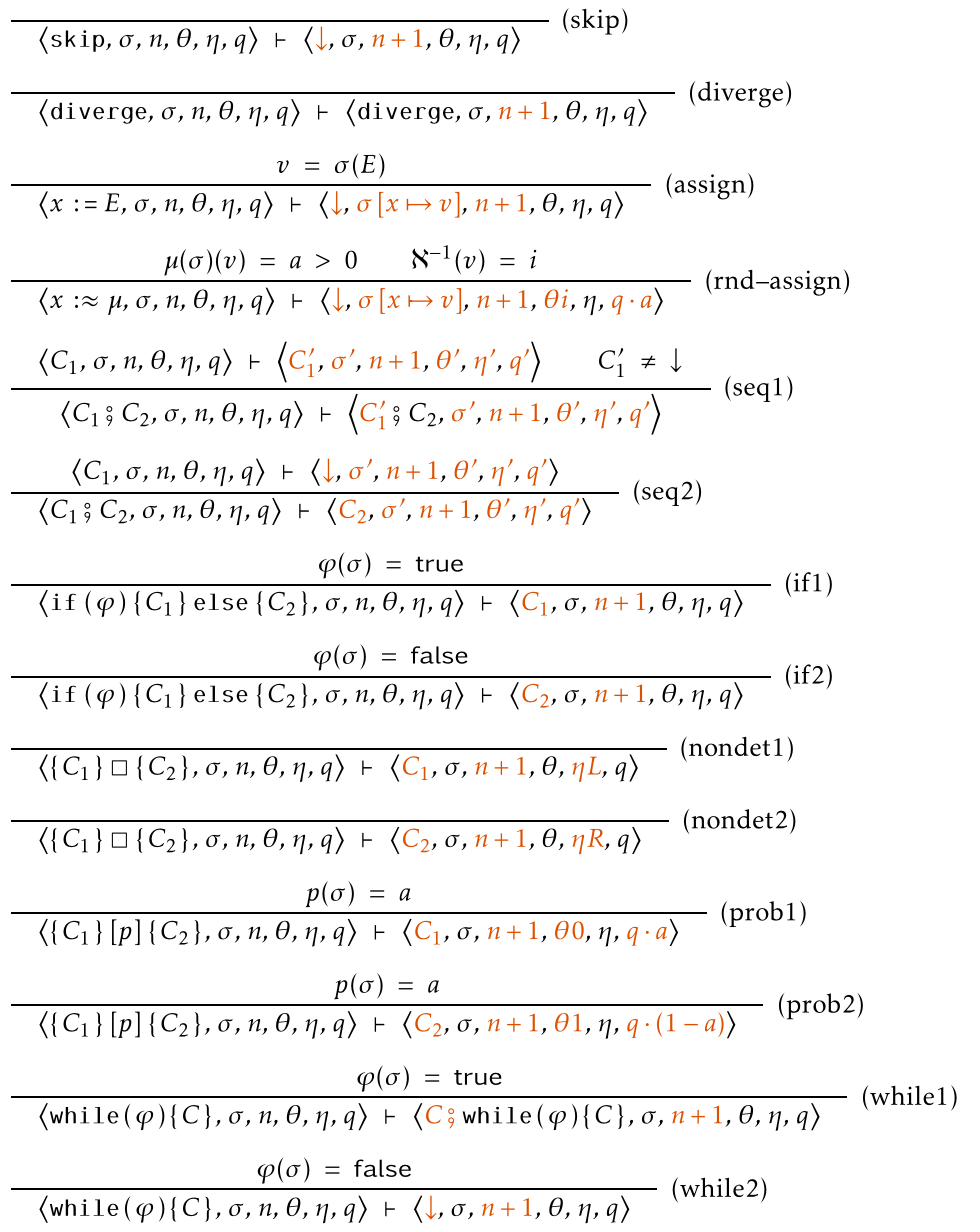
\includegraphics[height=1.2\textwidth]{pgcl-rel}
		\end{column}
		\begin{column}{0.5\textwidth}
			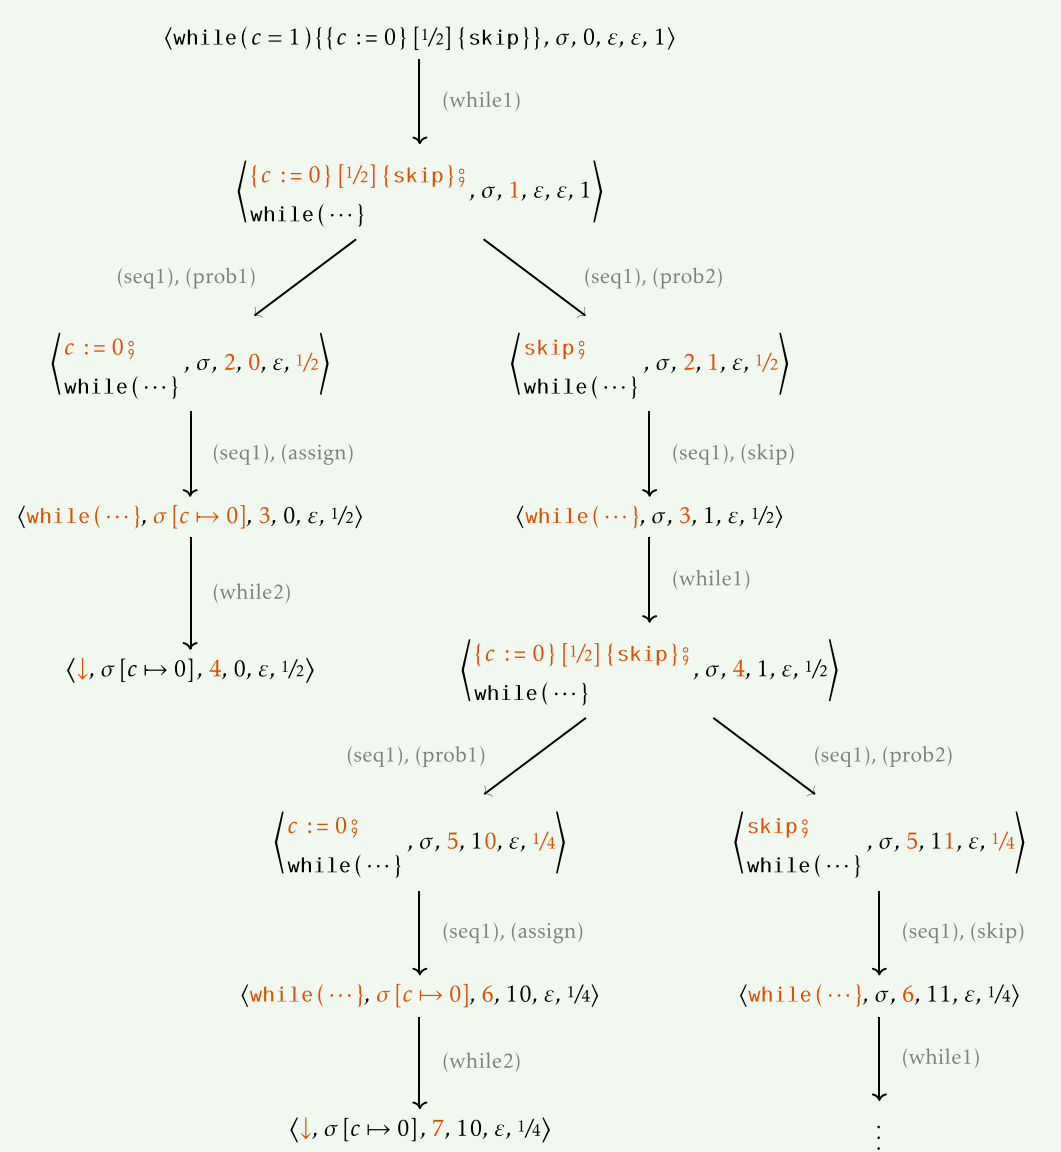
\includegraphics[height=1.1\textwidth]{pgcl-tree}
		\end{column}
	\end{columns}
\end{frame}
\subsection{Linear fragment of pGCL, ReDiP}
\begin{frame}{A fragement of pGCL: ReDiP}
	\begin{itemize}
		\item No divergence statement.
		\item All arithmetic expressions are linear/affine\\
		      \( a_0 + a_1 x_1 + a_2 x_2 \cdots a_n x_n \)
		      where \( a_i \in \mathbb{Z} \cup \PARMS \) and \( x_i \in \VARS \).
		\item All comparison expressions are rectangular\\
		      \(\langle expr \rangle\ op\ n\)
		      where \(op \in \{=,\neq,>,<.\leq,\geq\}\) and \(n\in \mathbb{Z}\cup\PARMS\).
		\item Special support for \(x \bmod 2 = 0\).
		\item Special support for IID sampling.
		\item Sampling from a user-defined PGF.
	\end{itemize}
	\hfill
	Still quite expressive :).
\end{frame}

\section{PGF transformer semantics}
\subsection{Review on PGFs}
\begin{frame}[allowframebreaks]{Generatingfuctionology\cite{gfbook}}
	\begin{block}{Notations}
		\begin{itemize}
			\item vectors \(\mathbf{x} = (x_1,x_2,\ldots x_k)\) and \(\sigma: \{1,\ldots,k\}\mapsto \mathbb{N}\)
			\item monomials \(\mathbf{x}^\sigma = x_1^{\sigma(1)} x_2^{\sigma(2)} \ldots x_k^{\sigma(k)} = \prod_i x_i^{\sigma(i)}\)
			\item polynomial rings \(\mathbb{R}\S{X}\), \(\mathbb{R}\S{X,Y}\), and \(\mathbb{R}\S{\mathbf{X}}\)
		\end{itemize}
	\end{block}
	\begin{block}{GF: sequences as formal power series}
		\[
			\sum_{n=0}^\infty a_n x^n
			\qquad
			\sum_{n=0}^\infty\sum_{m=0}^\infty b_{n,m} x^n y^m
			\qquad
			\sum_{\sigma \in\mathbb{N}^k}^\infty f(\sigma) \mathbf{x}^\sigma
		\]
	\end{block}
	\begin{block}{finite representation of infinite objects: closed-forms}
		\[
			\begin{array}{l|l|l}
				\hline
				\text{GF }g(x) & \text{seq }[x^n]g & \text{parameters}       \\
				\hline
				(1-ax)^k       & \binom{k}{n}a^n   & a,k\in\mathbb{R}^{\ast} \\
				(1-x)^{-2}     & n+1               &                         \\
				x^k            & [n=k]             & k\in\mathbb{N}^{+}      \\
				e^{kx}         & k^n/n!            & k\in\mathbb{R}^{\ast}   \\
				\ln(1+x)       & \frac{-1}{n}      & n\geq 1                 \\
			\end{array}
		\]
	\end{block}
	\begin{block}{sequence manipulation as algebraic operations}
		\centering
		\begin{tabular}{l|l}
			\hline
			sequence manipulation   & gf algebra             \\
			\hline
			\(a_{n-m}\)             & \(x^m f\)              \\
			\(a_{n} + b_{n}\)       & \(f+g\)                \\
			\(\alpha a_{n}\)        & \(\alpha f\)           \\
			\(\sum_k a_{k}b_{n-k}\) & \(fg\)                 \\
			\(n a_n\)               & \(x \partial_x f\)     \\
			\(a_{n-1}/n\)           & \(\int f \mathrm{d}x\) \\
			% an x^n -> n an x^(n-1) -> (n+1) a_{n+1} x^n
			% an x^n -> an/(n+1) x^(n+1) -> a{n-1}/n x^n
		\end{tabular}
	\end{block}

	\begin{exampleblock}{wikipedia/generating function/application/example 3}
		\[
			\begin{cases}
				U_n = 2V_{n-1} + U_{n-2} \\
				V_n = U_{n-1} + V_{n-2}  \\
				U_0=U_1=V_0=V_1=1
			\end{cases}
			\implies
			\begin{cases}
				U(z) = 1 + 2z V(z) + z^2 U(z) \\
				V(z) = zU(z)+z^2U(z) = \frac{z}{1-z^2}U(z)
			\end{cases}
		\]
		\[
			U(z)={\frac {1-z^{2}}{1-4z^{2}+z^{4}}}={\frac {1}{3-{\sqrt {3}}}}\cdot {\frac {1}{1-\left(2+{\sqrt {3}}\right)z^{2}}}+{\frac {1}{3+{\sqrt {3}}}}\cdot {\frac {1}{1-\left(2-{\sqrt {3}}\right)z^{2}}}
		\]
		\[
			U_{2n+1} = 0 \qquad U_{2n} = \left\lceil \frac{(2+\sqrt 3)^n}{3-\sqrt 3} \right\rceil
		\]
	\end{exampleblock}
\end{frame}
\begin{frame}[allowframebreaks]{Probability Generating Functions}
	Z-transform of PMF. \( \E(s^X) = \sum_n p(n) s^n\) and \( \E(s^X t^Y) = \sum_{n,m} p(n,m) s^n t^m \).
	\begin{block}{use of PGF}
		\begin{itemize}
			\item represent distributions using generating functions
			\item operating random variable is manipulating PGFs
			\item working in finite closed-form
		\end{itemize}
	\end{block}
	\begin{exampleblock}{Random stopping sum}
		A \(X_1, X_2, \ldots\) a sequence of iid variables with PGF \(g_X(\cdot)\). Another independent random variable \(N\) with PGF \(g_N(\cdot)\).
		\begin{align*}
			\E_{N,\mathbf{X}}\left\{ t^{\sum_{i=1}^N X_i} \right\}
			 & = \E_N\left\{ \E_{\mathbf{X}|N}\left[ t^{\sum_{i=1}^N X_i} \mid N \right] \right\}
			= \E_N\left\{ \E_{\mathbf{X}|N}\left[ \prod_{i=1}^N t^{X_i} \mid N \right] \right\}     \\
			 & = \E_N\left\{ \prod_{i=1}^N \E_{\mathbf{X}|N}\left[  t^{X_i} \mid N \right] \right\}
			= \E_N\left\{ \prod_{i=1}^N \E_{\mathbf{X}}\left[  t^{X_i} \right] \right\}
			= \E_N\left\{ {(g_X(t))}^N \right\}                                                     \\
			 & = \sum_{n=0}^{\infty} {(G_X(t))}^n \Pr(N=n)
			= g_N(g_X(t))
		\end{align*}
	\end{exampleblock}
\end{frame}

\subsection{PGF transformer semantics of ReDiP}
\begin{frame}[allowframebreaks]{PGF transformer semantics}
	\begin{block}{A denotational semantics}
		\begin{itemize}
			\item Distribution of program states represented as PGFs.
			\item Program executions transforms PGFs.
			\item A program is a PGF transformer \(\S{P}: \PGF\to\PGF\)
		\end{itemize}
	\end{block}

	Suppose that the program state is \(g = \mathbb{E}(s^X t^Y)\) where \(X,Y\in\mathbb{N}\):
	\begin{itemize}
		\item \texttt{x := n} assignment: \(g\mapsto g[s/1] s^n\)
		      \[
			      \mathbb{E}(s^X t^Y) \to s^n \mathbb{E}(1^X t^Y) = s^n \mathbb{E}(t^Y) = \mathbb{E}(s^n t^Y)
		      \]
		\item  \texttt{x := x+n} cumulation: \(g\mapsto g s^n\)
		      \[
			      \mathbb{E}(s^X t^Y) \to s^n \mathbb{E}(s^X t^Y) = \mathbb{E}(s^{X+n} t^Y)
		      \]
		\item  \texttt{x := x-1} self-decrement: \(g\mapsto (g-g[s/0])s^{-1} + g[s/0]\)
		      \[
			      \mathbb{E}(s^X t^Y) \to s^{-1}\mathbb{E}(s^X t^Y) = \mathbb{E}(s^{X-1} t^Y)
		      \]
		\item \texttt{x := x+y} addition: \(g\mapsto g[t/st]\)
		      \[
			      \mathbb{E}(s^X t^Y) \to \mathbb{E}(s^X (st)^Y) = \mathbb{E}(s^{X+Y} t^Y)
		      \]
		      \framebreak
		\item \texttt{x := D} samples from distribution: \(g\mapsto g[s/1] \cdot [D](s)\) where the PGF of \(D\) is \([D](r)\)
		      \[
			      \mathbb{E}(s^X t^Y) \to \mathbb{E}(s^D) \mathbb{E}(1^X t^Y) = \mathbb{E}(s^D t^Y)
		      \]
		\item \texttt{x := iid(D,y)} iid sampling: \(g\mapsto g[s/1][t/t[D](s)]\)
		      \[
			      \mathbb{E}(s^X t^Y) \to \mathbb{E}(1^X t^Y {([D](s))}^Y) = \sum_{0\leq m} {([D](s))}^m t^m
		      \]
		\item \texttt{if(x<n) \{P\} else \{Q\}} conditional branching: \( g\mapsto \S{P}(g_{x<n}) + \S{Q}(g-g_{x<n}) \) where
		      \[
			      g_{x<n} = \sum_{x<n} \sum_y p(x,y) s^x t^y = \sum_{i<n} \frac{s^i}{i!} \left(\frac{\partial^i}{\partial s^i}g\right)[s/0]
		      \]
		\item \texttt{P;Q} sequential composition: \(g\mapsto \S{Q}(\S{P}(g))\)
	\end{itemize}

	\begin{block}{make it sweet. syntactic sugar}
		\begin{center}
			\begin{tabular}{l|l}
				\hline
				\texttt{\{P\} [r] \{Q\}}                   & \(g\mapsto r\S{P}(g) + (1-r)\S{Q}(g)\)                      \\
				\hline
				\texttt{loop(n) \{P\}}                     & \(\S{P}(\S{P}\cdots \S{P}(g))\)                             \\
				\texttt{x := x-n}                          & \texttt{loop(n) \{x := x-1\}}                               \\
				\hline
				\texttt{if(\(p\land q\)) \{P\} else \{Q\}} & \texttt{if(\(p\))\{ if(\(q\))\{P\}else\{Q\} \} else\{Q\}}   \\
				\texttt{if(\(p\lor q\)) \{P\} else \{Q\}}  & \texttt{if(\(p\))\{P\} else \{ if(\(q\))\{P\} else\{Q\} \}} \\
				\texttt{if(\(\lnot p\)) \{P\} else \{Q\}}  & \texttt{if(\(p\)) \{Q\} else \{P\}}                         \\
				\hline
				\texttt{if(\(x\leq n\))  P else Q}         & \texttt{if(\(x<n+1\)) P else Q}                             \\
				\texttt{if(\(x> n\))     P else Q}         & \texttt{if(\(x\leq n\)) Q else P}                           \\
				\texttt{if(\(x\geq n\))  P else Q}         & \texttt{if(\(x<n\)) Q else P}                               \\
				\texttt{if(\(x =  n\))   P else Q}         & \texttt{if(\(x\leq n \land x \geq n\)) P else Q}            \\
				\texttt{if(\(x \neq n\)) P else Q}         & \texttt{if(\(\lnot (x=n)\)) P else Q}                       \\
				\hline
				\(x \bmod 2 = 0\)                          & \(g\mapsto \frac12(g[s/-s] + g)\)                           \\
				\(x \bmod 2 = 1\)                          & \(g\mapsto \frac12(g - g[s/-s])\)                           \\
				\hline
			\end{tabular}
		\end{center}
	\end{block}
\end{frame}

\subsection{Fixed point induction}
\begin{frame}[fragile]{The missing piece in PGF transformer semantics, loops}
	\begin{enumerate}
		\item A while loop
		      \( \mathrm{while}(\phi)\{P\} \)
		\item A infinitely nested braching tree
		      \begin{verbatim}
if(cond){
    body;
    if(cond){
        body;
        if(cond){
            body;
            ...
             ...
        }
    }
}\end{verbatim}
		\item A least fixed point
		      \( \mu X . \mathrm{if}(\phi)\{ P; X \} \)
	\end{enumerate}

	\begin{alertblock}{rigorous and complicated theoretical derivation}
		Not quite correct.
		\begin{itemize}
			\item The PRODIGY verifier only checks invariant instead of automatically infer one.
			\item Defining a \(\omega\)-complete partial order \((\leq,\PGF)\)
			\item For Almost Surely Termination (AST) programs:
			      \( \S{ \mathrm{if}(\phi)\{ P; X \} } \leq \S{ X } \)
			\item For Universally AST (UAST) programs:
			      \( \S{ \mathrm{if}(\phi)\{ P; X \} } = \S{ X } \)
		\end{itemize}
	\end{alertblock}
\end{frame}
\subsection{Properties of the PGF transformer semantics}
\begin{frame}{Linearity}
	For a well-formed ReDiP program \(P\), \(\S{P}\) is a linear transform
	\begin{itemize}
		\item \texttt{x := x+n} transformer \(g\mapsto s^n g\)
		      \[
			      (af + bg) \mapsto (af + bg)s^n = a(s^n f) + b(s^n g)
		      \]
		\item \texttt{x := x+y} transformer \(g\mapsto g[t/st]\)
		      \[
			      (af + bg) \mapsto (af + bg)[t/st] = a(f[t/st]) + b(g[t/st])
		      \]
		\item \texttt{x := 0} transformer \(g\mapsto g[s/1]\)
		      \[
			      (af + bg)[t/1] = af[t/1] + bg[t/1]
		      \]
		\item Other simple ReDiP program statements.
		\item By induction \texttt{P;Q} transformer \(g\mapsto \S{Q}(\S{P}(g))\).
		      \[
			      (af+bg) \mapsto \S{Q}(a\S{P}(f) + b\S{Q}(g)) = a\S{Q}(\S{P}(g)) + b \S{Q}(\S{P}(g))
		      \]
		\item Other compositonal statements \texttt{if(cond)\{P\}else\{Q\}} and \texttt{while(cond)\{P\}}.
	\end{itemize}
\end{frame}
\begin{frame}{Rational closed-form presevation}
	Rational closed-forms are amenable to computer algebra systems (e.g., sympy and GiNaC).
	\[
		\frac{f}{g} = \dfrac
		{ \sum_{i=0}^n\sum_{j=0}^m a_{ij} x^iy^j }
		{ \sum_{i=0}^n\sum_{j=0}^m b_{ij} x^iy^j }
	\]
	Rational closed-forms are closed under ReDiP transforms.
	\begin{itemize}
		\item \texttt{x := x+n} transformer \(g\mapsto s^n g\)
		      \[
			      \frac{f}{h} \mapsto \frac{s^n f}{h}
		      \]
		\item \texttt{x := x+y} transformer \(g\mapsto g[t/st]\)
		      \[
			      \frac{f}{h} \mapsto \frac{f[t/st]}{h[t/st]}
		      \]
		\item \texttt{x := 0} transformer \(g\mapsto g[s/1]\)
		      \[
			      \frac{f}{h} \mapsto \frac{f[s/1]}{h[s/1]}
		      \]
		\item Other simple ReDiP program statements.
		\item By induction \texttt{P;Q} transformer \(g\mapsto \S{Q}(\S{P}(g))\).
		      \[
			      f/h \mapsto \S{Q}(\S{P}(f/h)) = \S{Q}(f_1/h_1) = f_2/h_2
		      \]
		\item Other compositonal statements \texttt{if(cond)\{P\}else\{Q\}} and \texttt{while(cond)\{P\}}.
	\end{itemize}
\end{frame}

\subsection{PGF transformer equivalence}
\begin{frame}{Equivalence verification}
	For two ReDiP programs \(P_1,P_2\) whose state is \(g(X_1,X_2,\ldots X_n)\in\PGF(\mathbb{N}^n)\)

	\begin{itemize}
		\item Equivalence checking: for all valid generating function of distributions over \(\mathbb{N}^n\).\\
		      \(\displaystyle \forall g \in\PGF(\mathbb{N}^n) \quad \S{P_1}(g) = \S{P_2}(g) \)
		\item By linearity: for all pointmass distributions over \(\mathbb{N}^n\)\\
		      \(\displaystyle \forall (y_1,y_2,\ldots y_n) \in \mathbb{N}^n \quad \S{P_1}(X_1^{y_1}X_2^{y_2}\cdots X_n^{y_n}) = \S{P_2}(X_1^{y_1}X_2^{y_2}\cdots X_n^{y_n}) \)
		\item Ebbed all n-dim pointmass PGFs into a 2n-dim PGF \(\delta(\mathbf{X};\mathbf{U})\)\\
		      \(\displaystyle \S{P_1}(\delta) = \S{P_2}(\delta) \)
		      where
		      \(
		      \displaystyle
		      \delta
		      = \sum_{y_1,y_2,\ldots y_n} (U_1X_1)^{y_1}(U_2X_2)^{y_2}\cdots (U_nX_n)^{y_n}
		      = \prod_{i=1}^n \left( \sum_j (X_iU_i)^j \right)
		      = \prod_{i=1}^n (1-X_iU_i)^{-1}
		      \)
	\end{itemize}
\end{frame}
\begin{frame}{Summary}
	\begin{enumerate}
		\item Restricting syntax of pGCL to obtain ReDiP.
		\item Recursively defining the PGF transformer semantics of ReDiP.
		\item Handling unbounded loops with fixed-point induction.
		\item Equivalence checking leveraging linearity
	\end{enumerate}
\end{frame}

\section{Evaluation}
\subsection{Setup}
\begin{frame}{Benchmark setup}
	\begin{block}{Implementation}
		\begin{itemize}
			\item About 500 nlocs of Python implementation.
			\item pGCL analysis using the \emph{probably} package\cite{probably}.
			\item Algebraic computation with sympy\cite{sympy}.
		\end{itemize}
	\end{block}
	\begin{block}{Benchmark}
		15 pairs of equivalent programs from PRODIGY\cite{cav-pgf}.
	\end{block}
\end{frame}
\subsection{Results}
\begin{frame}[allowframebreaks]{Results}
	\begin{table}[htbp]
		\centering
		\caption{Results on the 15 test cases}
		\begin{tabular}{ll}
			\hline
			test case                        & time  \\
			\hline
			dep_bern.pgcl                    & 6.81s \\
			dueling_cowboys_parameter.pgcl   & 4.61s \\
			geometric.pgcl                   & 2.62s \\
			geometric_observe.pgcl           & 2.72s \\
			geometric_observe_parameter.pgcl & 4.90s \\
			geometric_parameter.pgcl         & 4.45s \\
			geometric_shifted.pgcl           & 6.18s \\
			ky_die.pgcl                      & 18.5s \\
			ky_die_2.pgcl                    & 3.96s \\
			ky_die_parameter.pgcl            & 26.0s \\
			n_geometric.pgcl                 & 2.37s \\
			negative_binomial_parameter.pgcl & 4.07s \\
			random_walk.pgcl                 & 4.46s \\
			running_paper_example.pgcl       & 2.36s \\
			trivial_iid.pgcl                 & 1.85s \\
			\hline
		\end{tabular}
	\end{table}

	\begin{table}[htbp]
		\centering
		\caption{scalability test: finite loop handling}
		\begin{tabular}{ll}
			\hline
			iterations & time    \\
			\hline
			1          & 2.75s   \\
			2          & 10.90s  \\
			3          & 19.36s  \\
			4          & 30.84s  \\
			5          & 43.52s  \\
			6          & 58.54s  \\
			7          & 72.68s  \\
			8          & 90.30s  \\
			9          & 105.35s \\
			10         & 122.72s \\
			\hline
		\end{tabular}
	\end{table}
\end{frame}

\subsection{Case Study}
\begin{frame}[fragile,allowframebreaks]{Case Study: \texttt{random_walk.pgcl}}
	\begin{itemize}
		\item Check result: equivalent. 7.340888474005624 seconds.
		\item Variables \(\{c\mapsto u_0x_0, s\mapsto u_1x_1, tmp\mapsto u_2x_2\}\) parameters \([]\)\\
		\item \(\S{P_1}(\delta)\): \texttt{(-u1*(u2*x2 - 1)*(u1*x0*sqrt(1 - x0**2) - u1*x0 + x0**2 - x0*(u1*sqrt(1 - x0**2) - u1 + x0) + 2*sqrt(1 - x0**2) - 2)/2 + (u2 - 1)*(u1*sqrt(1 - x0**2) - u1 + x0))/((u2 - 1)*(u0*x0 - 1)*(u2*x2 - 1)*(u1*sqrt(1 - x0**2) - u1 + x0))}
		\item \(\S{P_2}(\delta)\): \texttt{-u1*(sqrt(1 - x0**2) - 1)/(u0*u1*u2*x0*sqrt(1 - x0**2) - u0*u1*u2*x0 - u0*u1*x0*sqrt(1 - x0**2) + u0*u1*x0 + u0*u2*x0**2 - u0*x0**2 - u1*u2*sqrt(1 - x0**2) + u1*u2 + u1*sqrt(1 - x0**2) - u1 - u2*x0 + x0) + 1/((u0*x0 - 1)*(u2*x2 - 1))}
		\item Comparison \(\S{P_1}(\delta)-\S{P_2}(\delta)=0\)
	\end{itemize}

	\begin{columns}
		\begin{column}{0.5\textwidth}
			\begin{verbatim}
nat s; nat c; nat tmp;

while(s > 0){
    {s := s+1} [1/2] {s := s-1}
    c := c+1
    tmp := 0
} \end{verbatim}
		\end{column}
		\begin{column}{0.5\textwidth}
			\begin{verbatim}
nat s; nat c; nat tmp;

if(s > 0){
    tmp := iid( ((1-(1-(c*c))^(1/2))/c), s)
    c := c + tmp
    tmp := 0; s := 0
} else { skip } \end{verbatim}
		\end{column}
	\end{columns}
\end{frame}

\section{Discussion}
\subsection{Conclusion of this project}

\begin{frame}{Conclusion}
	Our contributions:
	\begin{itemize}
		\item We define ReDiP a simple yet expressive subset of pGCL.
		\item We present the PGF transformers semantics of ReDiP.
		\item We explain the properties of PGF transformers.
		\item We designed an algorithm for ReDiP equivalence checking based on PGF transformer semantics.
		\item We tested the effectiveness and efficiency of such tool.
	\end{itemize}
\end{frame}
\subsection{Future works}

\begin{frame}[fragile, allowframebreaks]{Limitations and future works}
	\begin{block}{conditional equivalence checking}
		From \(\S{P_1} = \S(P_2)\) to \(\S{P_1|\phi} = \S{P_2|\phi}\)
		\begin{verbatim}
-- prog: a program that handles input x such that P(x) is true
-- cond: the P(x) predicate
restrict :: (a -> Bool) -> (a -> b) -> (a -> Maybe b)
restrict cond prog input = if cond input
                           then Just (prog input)
                           else Nothing
-- check equivalence: (restrict p f) (restrict p g)
			\end{verbatim}

		Obstacles:
		\begin{itemize}
			\item Support for conditional reasoning (\texttt{observe(..)} in pGCL).
			\item Expressing conditions besides rectangular ones, e.g., \(x^2 + y^2 < 1\).
		\end{itemize}
	\end{block}

	\begin{block}{incorporating real-valued variables using MGF/CF}
		Discrete random variables likes \(\operatorname{Poisson}(\lambda)\) and \(\operatorname{Binomial}(n,p)\) are not enough.
		How to add support for \(\mathcal{N}(\mu,\sigma^2)\) and \(\beta(\alpha,\beta)\)?\\

		A natural generalization would be:
		\begin{align*}
			\E(e^{sX + tY}) & \to e^{cs} \E(e^{0X + tY}) = \E(e^{sc + tY}) \\
			\E(e^{sX + tY}) & *\to \E(e^{sX + (t+s)Y}) = \E(e^{s(X+Y) tY}) \\
		\end{align*}

		Obstacles:
		\begin{itemize}
			\item Rational closed-form preservation no longer holds.
			\item Rectangular bound $x<c$ hard to express for MGF/CF
			      \begin{align*}
				      \E(t^{X I(X<n)})  & = \sum_{x<n} p(x=n) t^n                      \\
				      \E(e^{tX I(X<n)}) & = \int_{-\infty}^{c} f(x) e^{tx} \mathrm{d}x \\
			      \end{align*}
		\end{itemize}
	\end{block}

	\begin{block}{reactive programs}
		\begin{itemize}
			\item The current approach works for UAST programs.
			\item Reactive programs are naturally non-terminating.
			\item Possible solution: bisimulation based equivalence checking.
		\end{itemize}
		\begin{columns}
			\begin{column}{0.5\textwidth}
				\begin{verbatim}
OnInputSymbol(() => {
    alpha1, alpha2 = iid(std_normal, 2)
    x[n] = input();
    output(alpha1 * (x[n-1] - mu) 
          + alpha2 * (x[n-2] - mu)^2);
    mu = (mu * n + x[n]) / (n + 1);
    n += 1;
})\end{verbatim}
			\end{column}
			\begin{column}{0.5\textwidth}
				\begin{verbatim}
OnInputSymbol(() => {
    alpha1, alpha2 = iid(std_normal, 2)
    output(alpha1 * (x[n-1] - mu) 
          + alpha2 * (x[n-2]^2 
             - 2*x[n]*mu + mu^2));
    x[n] = input();
    n += 1
    mu = (mu * (n-1) + x[n]) / n
})\end{verbatim}
			\end{column}
		\end{columns}
	\end{block}
\end{frame}

\appendix

\begin{frame}[allowframebreaks]{references}
	\nocite{*}
	\printbibliography
\end{frame}

\begin{frame}{Q and A}
	\begin{center}
		Questions are welcomed.
	\end{center}
\end{frame}

\end{document}
\end{document}
